%%%%%%%%%%%%%%%%%%%%%%%%%%%%%%%%%%%%%%%%%
% baposter Landscape Poster
% LaTeX Template
% Version 1.0 (11/06/13)
%
% baposter Class Created by:
% Brian Amberg (baposter@brian-amberg.de)
%
% This template has been downloaded from:
% http://www.LaTeXTemplates.com
%
% License:
% CC BY-NC-SA 3.0 (http://creativecommons.org/licenses/by-nc-sa/3.0/)
%
%%%%%%%%%%%%%%%%%%%%%%%%%%%%%%%%%%%%%%%%%

%----------------------------------------------------------------------------------------
%	PACKAGES AND OTHER DOCUMENT CONFIGURATIONS
%----------------------------------------------------------------------------------------

%\documentclass[landscape,a0paper,fontscale=0.285]{baposter} % Adjust the font scale/size here
\documentclass[landscape,a0paper,fontscale=0.285]{baposter}
\usepackage{epstopdf}
\usepackage{boolexpr}
\usepackage{graphicx} % Required for including images
\graphicspath{{figures/}} % Directory in which figures are stored
\usepackage{amsmath} % For typesetting math
\usepackage{amssymb} % Adds new symbols to be used in math mode

\usepackage{booktabs} % Top and bottom rules for tables
\usepackage{setspace}
\usepackage{array}
\newcolumntype{L}[1]{>{\raggedright\arraybackslash}p{#1}}
\usepackage{enumitem} % Used to reduce itemize/enumerate spacing
\usepackage{palatino} % Use the Palatino font
\usepackage[font=small,labelfont=bf]{caption} % Required for specifying captions to tables and figures

\usepackage{multicol} % Required for multiple columns
\setlength{\columnsep}{1.5em} % Slightly increase the space between columns
\setlength{\columnseprule}{0mm} % No horizontal rule between columns

\usepackage{tikz} % Required for flow chart
\usetikzlibrary{shapes,arrows} % Tikz libraries required for the flow chart in the template

\newcommand{\compresslist}{ % Define a command to reduce spacing within itemize/enumerate environments, this is used right after \begin{itemize} or \begin{enumerate}
\setlength{\itemsep}{1pt}
\setlength{\parskip}{0pt}
\setlength{\parsep}{0pt}
}

\definecolor{lightblue}{rgb}{0.145,0.6666,1} % Defines the color used for content box headers
\definecolor{darkred}{cmyk}{0,.85,.75,.3}
\definecolor{Blue}{rgb}{0,0,1}
\newcommand\A{{\bf\color{red} A }}
\newcommand\B{{\bf\color{Blue} B }}	
\newcommand{\Assumption}[1]{
 \switch[#1]
  \case{=1} Consistent representation between individuals %
  \case{=2} Local representations within an individual %
  \case{=3} Local representations between individuals %
  \case{=4} Independence %
  \case{=5} Representation is sparse %
  \case{=6} Representation is redundant %
 \endswitch  	
}
\newcommand{\Description}[1]{
 \switch[#1]
  \case{=1} A given unit within a particular representation will respond to various stimuli in the same way across individuals. %
  \case{=2} In any individual, anatomically neighboring units likely contribute to the same representation. %
  \case{=3} Across individuals, the units that contribute to a given representation will be found in similar anatomical locations. %
  \case{=4} The information coded by a unit activation does ot depend on the activation of other units. %
  \case{=5} Of all units measures, only a small proportion will be involved in the representation of interest. %
  \case{=6} The responses of units within a representation are highly correlated. %
 \endswitch  	
}
\begin{document}

\begin{poster}
{
columns=3,
grid=true,
headerborder=closed, % Adds a border around the header of content boxes
colspacing=1em, % Column spacing
bgColorOne=white, % Background color for the gradient on the left side of the poster
bgColorTwo=white, % Background color for the gradient on the right side of the poster
borderColor=black, % Border color
headerColorOne=darkred, % Background color for the header in the content boxes (left side)
headerColorTwo=darkred, % Background color for the header in the content boxes (right side)
headerFontColor=white, % Text color for the header text in the content boxes
boxColorOne=white, % Background color of the content boxes
textborder=roundedleft, % Format of the border around content boxes, can be: none, bars, coils, triangles, rectangle, rounded, roundedsmall, roundedright or faded
eyecatcher=true, % Set to false for ignoring the left logo in the title and move the title left
headerheight=0.1\textheight, % Height of the header
headershape=roundedright, % Specify the rounded corner in the content box headers, can be: rectangle, small-rounded, roundedright, roundedleft or rounded
headerfont=\Large\bf\textsc, % Large, bold and sans serif font in the headers of content boxes
%textfont={\setlength{\parindent}{1.5em}}, % Uncomment for paragraph indentation
linewidth=2pt % Width of the border lines around content boxes
}
%----------------------------------------------------------------------------------------
%	TITLE SECTION 
%----------------------------------------------------------------------------------------
%
{
\includegraphics[height=4em]{UWlogo_warm.eps}} % First university/lab logo on the left
{\bf\textsc{Unnecessarily Complicated Research Title}\vspace{0.5em}} % Poster title
{\textsc{\{ John Smith, James Smith and Jane Smith \} \hspace{12pt} University and Department Name}} % Author names and institution
{
\includegraphics[height=4em]{UWlogo_cool.eps}} % Second university/lab logo on the right

%----------------------------------------------------------------------------------------
%	INTRODUCTION
%----------------------------------------------------------------------------------------

\headerbox{Introduction}{name=intro,column=0,row=0}{

\begin{itemize}\compresslist

\item {\bf PDP models} have motivated many influential hypotheses. 

\item {\bf Distributed representations} are at the heart, responsible the learning, responding, generalizing, and predicting that the modes are capable of.

\item However, there is {\bf limited neural evidence}for distributed representations, e.g. from fMRI.

\item There may be a disconnect between methods of analysis and representational assumptions of PDP that {\bf systematically overlook} distributed patterns in the brain. 

\item {\bf SOS LASSO} is an optimization technique that is sensitive to distributed representations, {\em similarly located} in {\em samples of subjects}. 

\end{itemize}

\vspace{0.3em} % When there are two boxes, some whitespace may need to be added if the one on the right has more content
}

%----------------------------------------------------------------------------------------
%	DATA GENERATION & METHOD
%----------------------------------------------------------------------------------------

\headerbox{Data Generation \& Method}{name=objectives,column=0,below=intro}{
Data were generated by training an auto-encoder neural network.
\begin{itemize}\compresslist
\item Two areas specified to be \A and \B selective.
\item One area placed between systematic input and output units.
\item Categorization is possible based on either region, but the information is represented very differently.
\end{itemize}

\begin{center}
{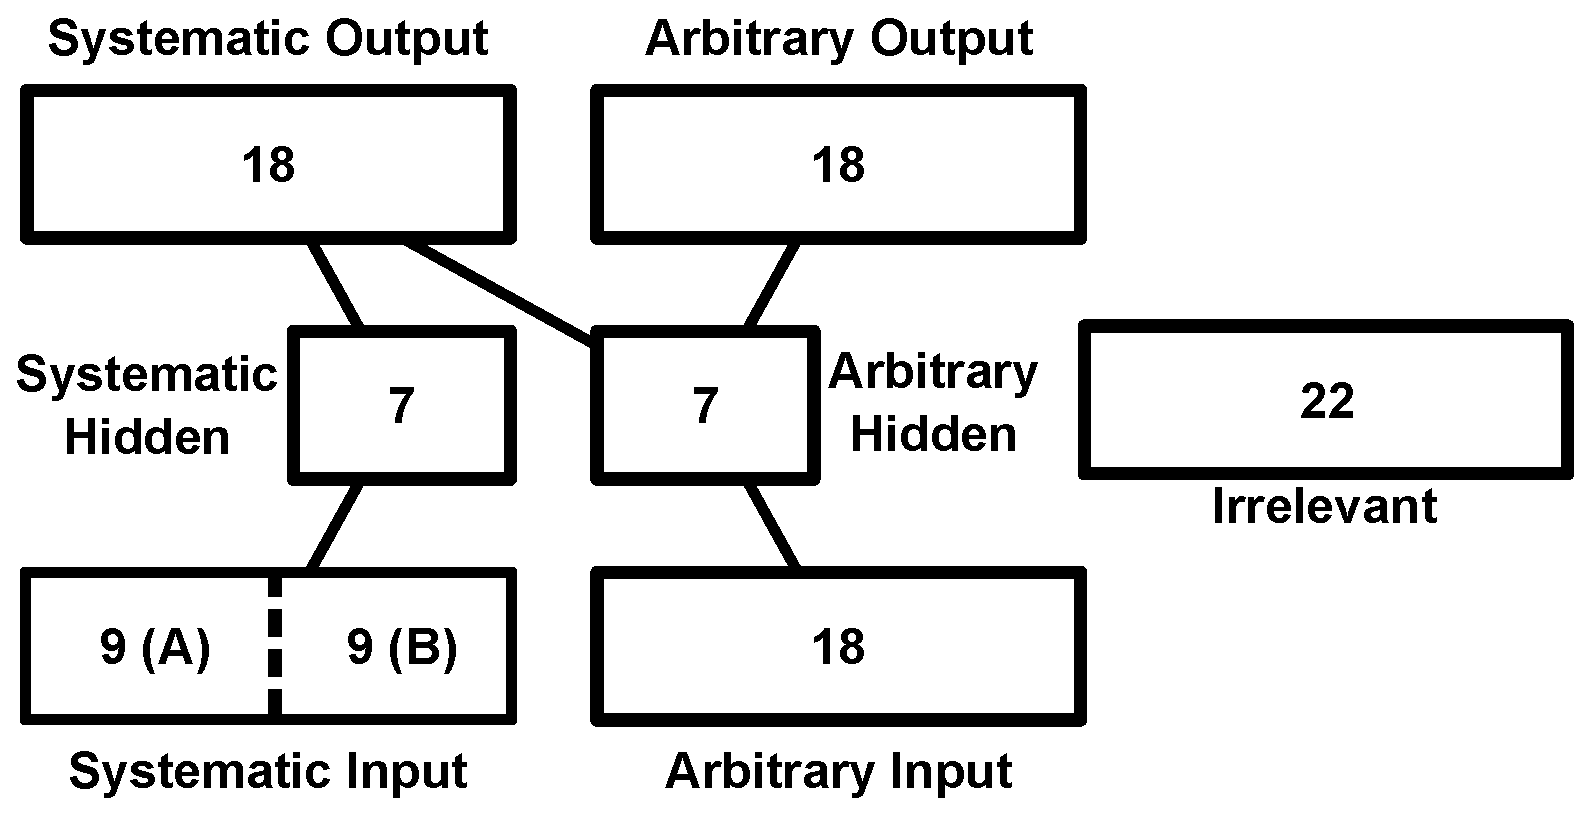
\includegraphics[width=0.55\textwidth]{model_outline.eps}}
{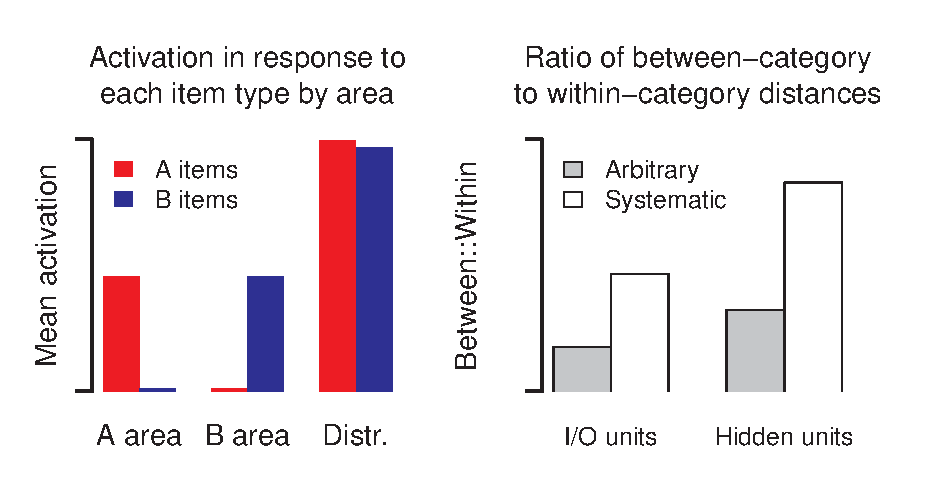
\includegraphics[width=0.75\textwidth]{activation_vs_distance.eps}}
\end{center}

{\bf Methods vary in their representational assumptions, and will label different patterns of data as ``important''.} We explore this by applying a range of methods to these data, to obviate the consequences of these assumptions.
}

%----------------------------------------------------------------------------------------

%----------------------------------------------------------------------------------------
%	 GENERATION
%----------------------------------------------------------------------------------------

\headerbox{Data Generation}{name=objectives,column=1,row=0}{
Data were generated by training an auto-encoder neural network.
\begin{itemize}\compresslist
\item Two areas specified to be \A and \B selective.
\item One area placed between systematic input and output units.
\item Categorization is possible based on either region, but the information is represented very differently.
\end{itemize}

\begin{center}
{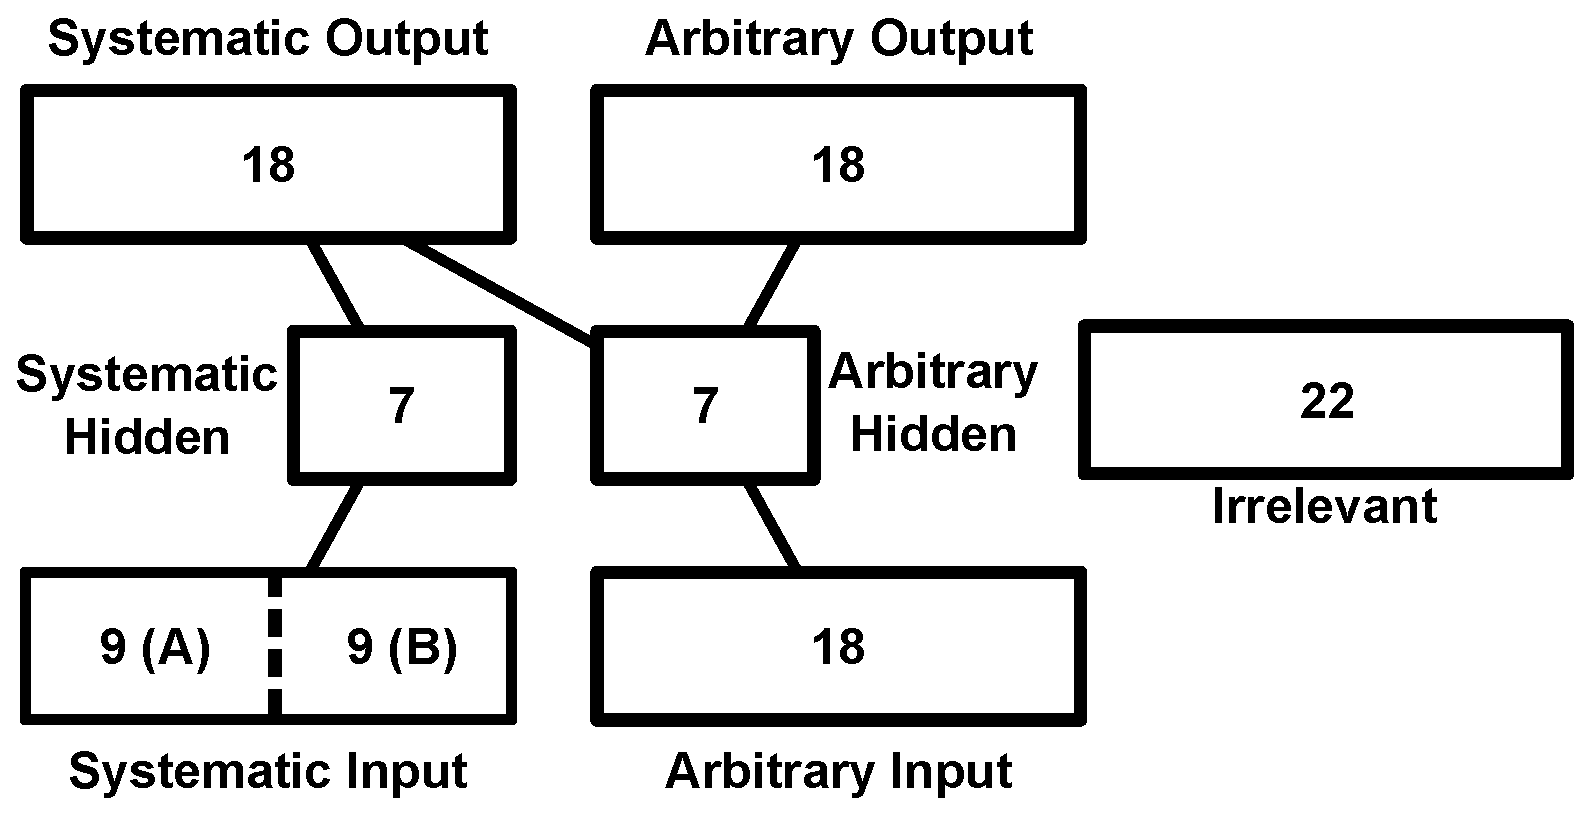
\includegraphics[width=0.55\textwidth]{model_outline.eps}}
{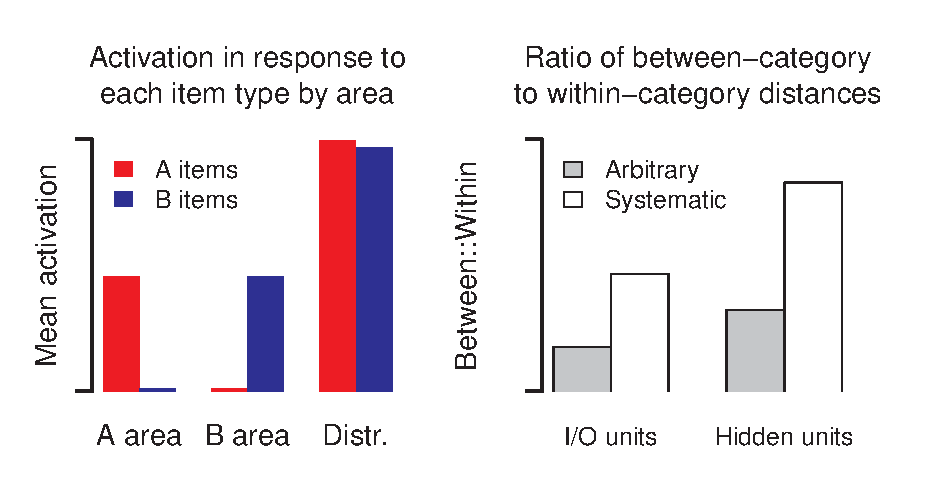
\includegraphics[width=0.75\textwidth]{activation_vs_distance.eps}}
\end{center}

{\bf Methods vary in their representational assumptions, and will label different patterns of data as ``important''.} We explore this by applying a range of methods to these data, to obviate the consequences of these assumptions.
}

%----------------------------------------------------------------------------------------

\end{poster}

\end{document}